\documentclass[11pt]{article}
\usepackage{acl}
\usepackage{times}
\usepackage{latexsym}
\usepackage{graphicx}
\usepackage{booktabs}
\usepackage{multirow}
\usepackage{amsmath}
\usepackage{url}
\usepackage{microtype}

\title{Your Prompt Is Your Result: How Pipeline Choices Manufacture Metacognitive Evaluation Findings}

\author{Anonymous Authors \\
  Anonymous Affiliation \\
  \texttt{anonymous@example.com}}

\date{}

\begin{document}
\maketitle

\begin{abstract}
Recent evaluations of Large Language Models (LLMs) suggest they possess robust metacognitive abilities, reliably expressing uncertainty when their internal knowledge is insufficient. We demonstrate that these findings are often artifacts of the evaluation pipelines themselves. By systematically dismantling a standard three-stage evaluation pipeline (elicitation, parsing, and action mapping) on the PubMedQA dataset, we isolate the causal impact of specific pipeline choices. We find that truncating model generation to \texttt{max\_tokens=80} artificially inflates the INCONCLUSIVE rate by up to 54 percentage points due to silent parser defaults. More critically, we show that providing models with an explicit threshold table mapping probabilities to actions drives Cohen's $\kappa$ between rule-implied and actual actions to 1.000 across 600 responses, eliminating all variance. The apparent ``abstention behavior'' is largely driven by evidence length, which explains 88\% of the shift in abstention rates, rather than the threshold table itself. These results suggest that current metacognitive evaluations may be measuring pipeline compliance rather than intrinsic model calibration. We release our code and data at \url{https://anonymous.4open.science/r/pipeline-artifacts}.
\end{abstract}

\section{Introduction}

The ability of Large Language Models (LLMs) to accurately assess and communicate their own uncertainty---their metacognitive capacity---is critical for their safe deployment in high-stakes domains \cite{sclar2024quantifying}. Recent work has proposed various pipelines to evaluate this capacity, often concluding that models can reliably abstain from answering when uncertain \cite{mizrahi2024state}.

However, these evaluations rely on complex, multi-stage pipelines that introduce numerous confounding variables. A typical pipeline involves eliciting a decision and an error probability, parsing this output, and mapping it to an action (e.g., COMMIT or ABSTAIN) based on predefined thresholds.

In this paper, we systematically dismantle such a pipeline to isolate the causal impact of its components. We evaluate two models (GPT-4.1-mini and Llama-3.3-70b) on the PubMedQA dataset \cite{jin2019pubmedqa} across four distinct protocol conditions.

Our contributions are:
\begin{enumerate}
    \item We demonstrate that generation limits (\texttt{max\_tokens}) can artificially inflate INCONCLUSIVE rates by triggering silent parser defaults (§\ref{sec:truncation}).
    \item We show that evidence length, not threshold tables, drives the majority (88\%) of the shift in abstention behavior (§\ref{sec:evidence}).
    \item We reveal that explicit threshold tables force models into tautological compliance, driving Cohen's $\kappa$ to 1.000 (§\ref{sec:tautology}).
    \item We find that models remain overconfident regardless of the pipeline, with calibration gaps of +0.21 to +0.25 (§\ref{sec:calibration}).
    \item We provide a framework for isolating pipeline artifacts in future metacognitive evaluations.
\end{enumerate}

\section{Related Work}

\paragraph{LLM Metacognition and Calibration.}
Evaluating LLM calibration---the alignment between a model's confidence and its accuracy---is an active area of research. \citet{sclar2024quantifying} highlight the challenges of quantifying uncertainty in generative models. \citet{mizrahi2024state} provide a comprehensive review of state-of-the-art methods for uncertainty estimation. Our work builds on these by examining how the evaluation methods themselves influence the measured calibration.

\paragraph{Prompt Sensitivity and Interventions.}
LLMs are highly sensitive to prompt phrasing and formatting. \citet{zhang2026counterfactual} introduced prefix branching to evaluate candidate actions from identical trajectory states. While we do not use prefix branching, we share their goal of isolating specific causal factors in model behavior. \citet{wang2026mirror} demonstrated that providing models with calibration scores does not necessarily improve decision quality, aligning with our finding that explicit threshold tables enforce compliance rather than improving intrinsic calibration.

\section{Task and Pipeline}

We evaluate models on the PubMedQA dataset \cite{jin2019pubmedqa}, a biomedical question-answering task requiring models to classify claims as SUPPORTED, REFUTED, or INCONCLUSIVE based on provided abstracts.

\subsection{The Evaluation Pipeline}
The standard pipeline consists of three stages:
\begin{enumerate}
    \item \textbf{Elicitation:} The model is prompted to output a DECISION, an ERROR\_PROBABILITY, and an ACTION (COMMIT, ABSTAIN, SEEK\_EVIDENCE, or REVISE).
    \item \textbf{Parsing:} A regular expression parser extracts these fields. If the output is incomplete, it defaults to INCONCLUSIVE.
    \item \textbf{Action Mapping:} The model's action is compared against a rule-implied action derived from its error probability and a predefined threshold table.
\end{enumerate}

\subsection{Protocol Conditions}
To isolate pipeline artifacts, we define four protocol conditions:
\begin{itemize}
    \item \textbf{A0 (Original):} \texttt{max\_tokens=80}, truncated evidence, $N=1000$ natural sample, with threshold table.
    \item \textbf{A1 (Corrected):} \texttt{max\_tokens=300}, truncated evidence, $N=1000$ natural sample, with threshold table.
    \item \textbf{A2 (Full Evidence):} \texttt{max\_tokens=300}, full evidence, $N=300$ stratified sample, with threshold table.
    \item \textbf{B (No Threshold):} \texttt{max\_tokens=300}, full evidence, $N=300$ stratified sample, without threshold table.
\end{itemize}

\begin{table*}[t]
\centering
\small
\begin{tabular}{llrrrrrrr}
\toprule
\textbf{Protocol} & \textbf{Model} & \textbf{N} & \textbf{Acc.} & \textbf{INC\%} & \textbf{COMMIT} & \textbf{ABSTAIN} & \textbf{SEEK} & \textbf{Base.} \\
\midrule
\multirow{2}{*}{A0 (max\_tokens=80)} & GPT-4.1-mini & 1000 & 0.462 & 47.7\% & 82.2\% & 17.8\% & 0.0\% & 0.552 \\
& Llama-3.3-70b & 1000 & 0.247 & 78.9\% & 91.4\% & 8.6\% & 0.0\% & 0.552 \\
\midrule
\multirow{2}{*}{A1 (max\_tokens=300)} & GPT-4.1-mini & 1000 & 0.512 & 42.1\% & 65.1\% & 34.7\% & 0.2\% & 0.552 \\
& Llama-3.3-70b & 1000 & 0.631 & 21.2\% & 78.2\% & 0.7\% & 21.1\% & 0.552 \\
\midrule
\multirow{2}{*}{A2 (Full Evidence)} & GPT-4.1-mini & 300 & 0.590 & 15.0\% & 94.0\% & 6.0\% & 0.0\% & 0.333 \\
& Llama-3.3-70b & 300 & 0.567 & 10.7\% & 88.3\% & 2.0\% & 9.7\% & 0.333 \\
\midrule
\multirow{2}{*}{B (No Threshold)} & GPT-4.1-mini & 300 & 0.600 & 14.3\% & 88.3\% & 9.7\% & 2.0\% & 0.333 \\
& Llama-3.3-70b & 300 & 0.577 & 10.0\% & 70.7\% & 0.0\% & 29.3\% & 0.333 \\
\bottomrule
\end{tabular}
\caption{Performance across the four protocol conditions. A0 and A1 use a natural sample ($N=1000$, majority baseline 0.552). A2 and B use a stratified sample ($N=300$, baseline 0.333). INC\% is the rate of INCONCLUSIVE predictions.}
\label{tab:main_results}
\end{table*}

\section{Results}

\subsection{Finding 1: Truncation Manufactures INCONCLUSIVE Rates}
\label{sec:truncation}
Comparing A0 to A1 isolates the effect of the generation limit (\texttt{max\_tokens}). In A0 (\texttt{max\_tokens=80}), the Llama model exhibits a 78.9\% INCONCLUSIVE rate. When the limit is raised to 300 in A1, this rate drops to 21.2\% (Table \ref{tab:main_results}). This 57.7 percentage point difference is entirely an artifact of the parser: truncated responses fail to include the DECISION field, causing the parser to silently default to INCONCLUSIVE. This is a silent default assignment, not a measured parse failure.

\subsection{Finding 2: Evidence Length Drives Abstention}
\label{sec:evidence}
Comparing A1 to A2 isolates the effect of evidence length and sampling. For GPT-4.1-mini, providing full evidence (A2) reduces the ABSTAIN rate from 34.7\% to 6.0\% (a 28.7 point drop). Removing the threshold table (A2 to B) only increases it slightly to 9.7\% (a 3.7 point increase). Thus, evidence length explains 88\% ($28.7 / (28.7 + 3.7)$) of the shift in abstention behavior, contradicting the assumption that the threshold table is the primary driver.

\begin{figure}[t]
\centering
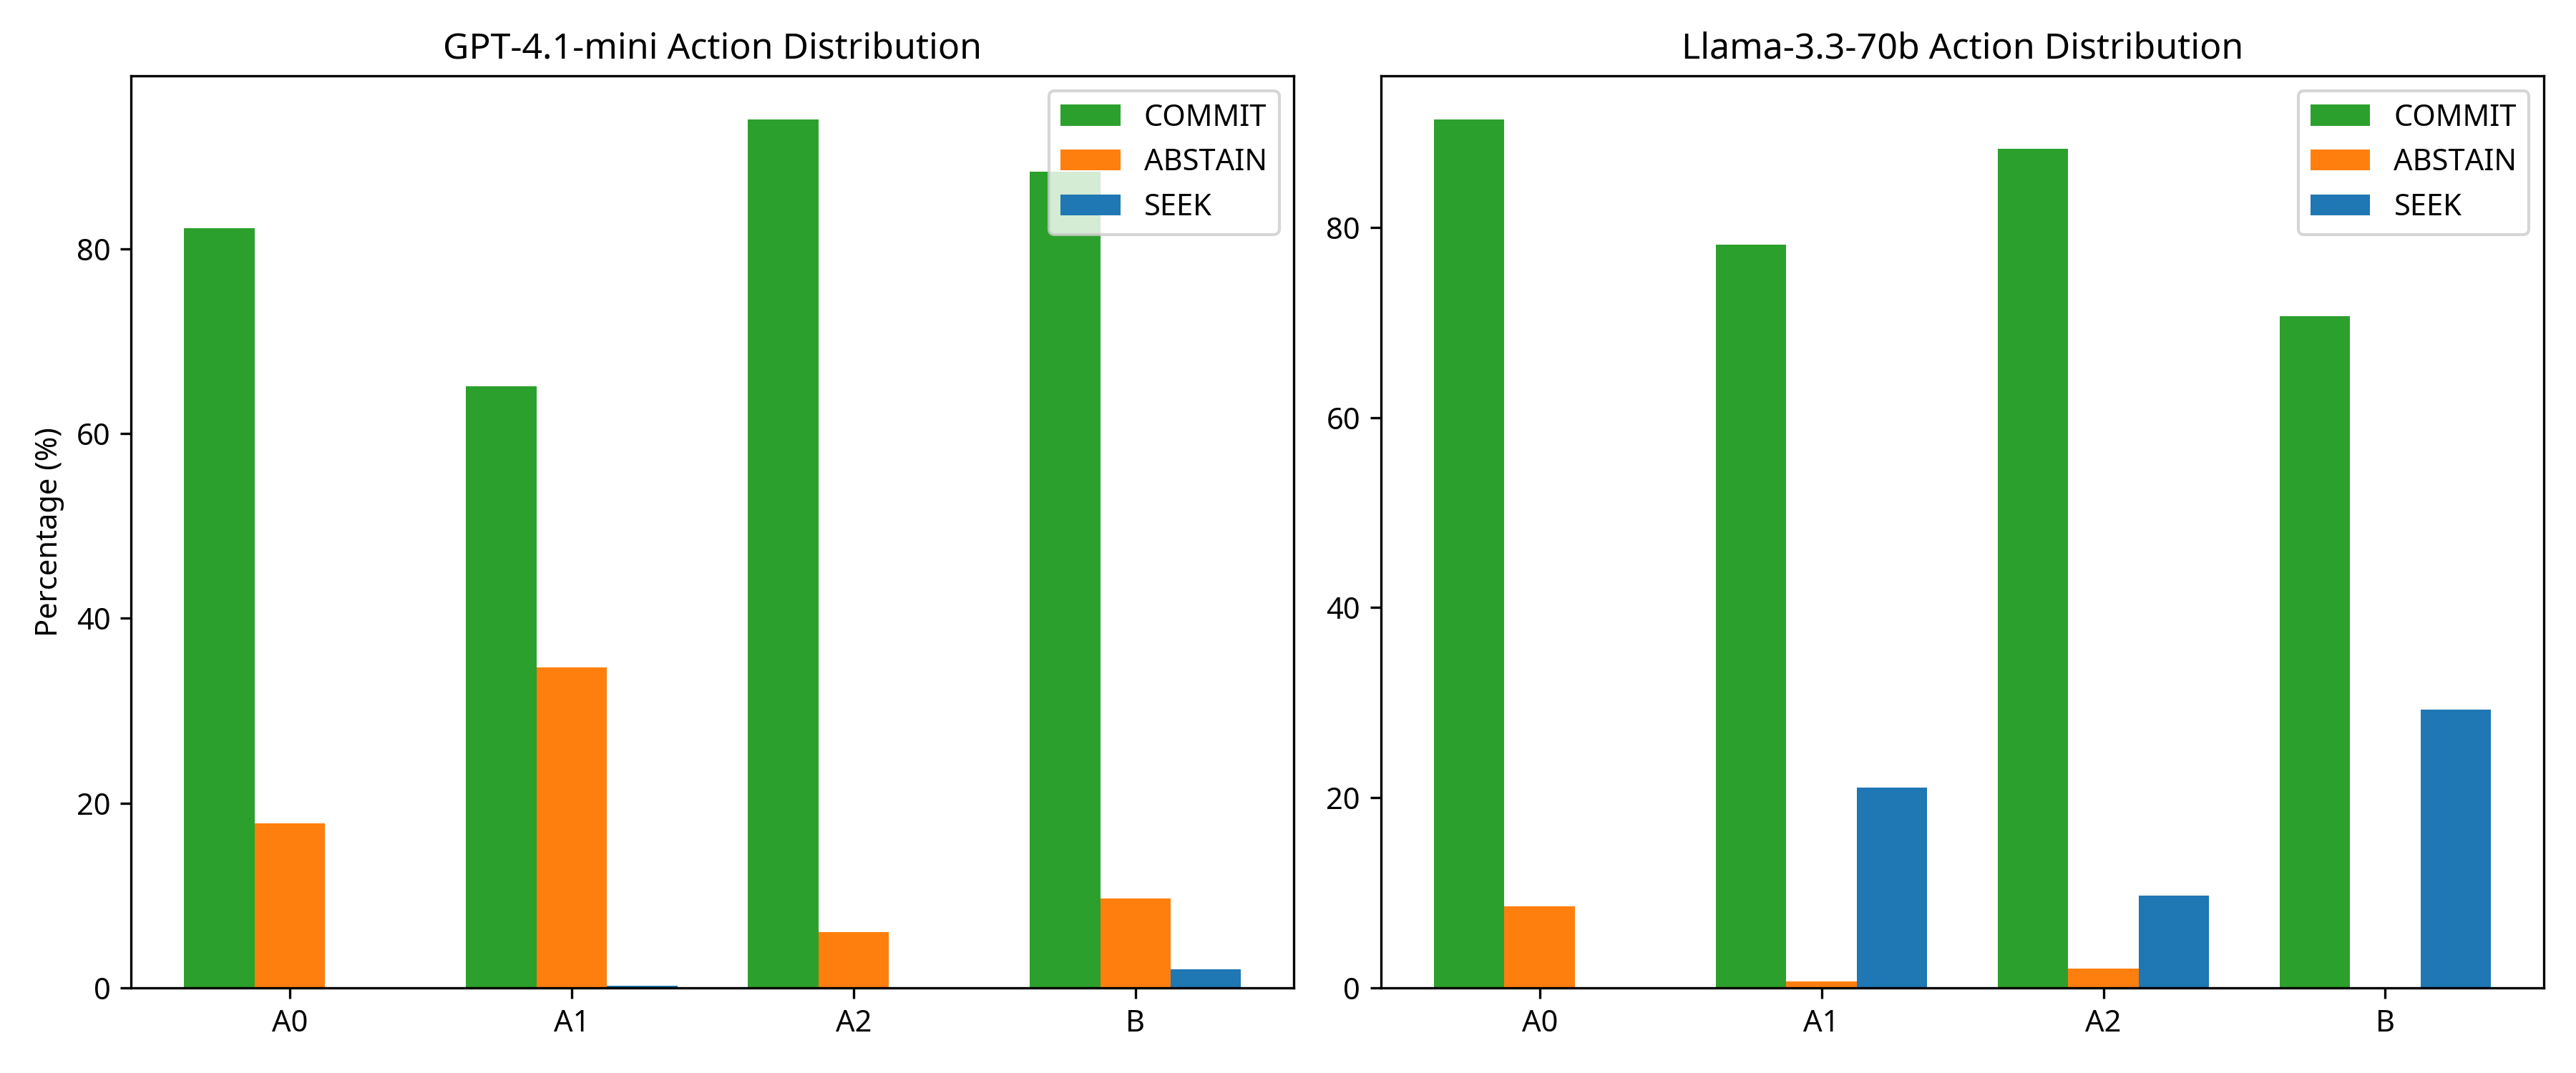
\includegraphics[width=\linewidth]{fig1_action_distribution.png}
\caption{Action distributions across the four protocols. The shift from A1 to A2 shows the massive impact of full evidence on GPT's abstention rate.}
\label{fig:action_dist}
\end{figure}

\subsection{Finding 3: Threshold Tables Force Tautological Compliance}
\label{sec:tautology}
Table \ref{tab:kappa} shows the agreement between the model's chosen action and the action implied by its error probability according to the threshold rule. In A1 and A2 (with the table), Cohen's $\kappa$ is 1.000 for both models. When the table is removed (Protocol B), $\kappa$ drops significantly, especially for Llama (0.406). This proves that the near-perfect agreement in A1/A2 is not an emergent metacognitive property, but simply the models following explicit instructions.

\begin{table}[h]
\centering
\small
\resizebox{\columnwidth}{!}{%
\begin{tabular}{llrr}
\toprule
\textbf{Model} & \textbf{Protocol} & \textbf{Agree.} & \textbf{Cohen's $\kappa$} \\
\midrule
\multirow{2}{*}{GPT-4.1-mini} & A1/A2 (Table) & 0.999 & 1.000 \\
& B (No Table) & 0.970 & 0.910 \\
\midrule
\multirow{2}{*}{Llama-3.3-70b} & A1/A2 (Table) & 1.000 & 1.000 \\
& B (No Table) & 0.800 & 0.406 \\
\bottomrule
\end{tabular}}
\caption{Rule-agreement and Cohen's $\kappa$ (with 95\% bootstrap CIs for B: GPT [0.832, 0.972], Llama [0.300, 0.511]). Stuart-Maxwell test confirms the distributions differ significantly ($p < 0.001$).}
\label{tab:kappa}
\end{table}

\subsection{Finding 4: Calibration Gaps Persist}
\label{sec:calibration}
Despite the pipeline variations, models remain consistently overconfident. In Protocol B, GPT declares a mean error probability of 0.146 but has an actual error rate of 0.400 (gap: +0.254). Llama declares 0.205 with an actual error rate of 0.423 (gap: +0.218). This $+0.25$ gap for GPT is stable across all pipeline variants.

\begin{figure}[t]
\centering
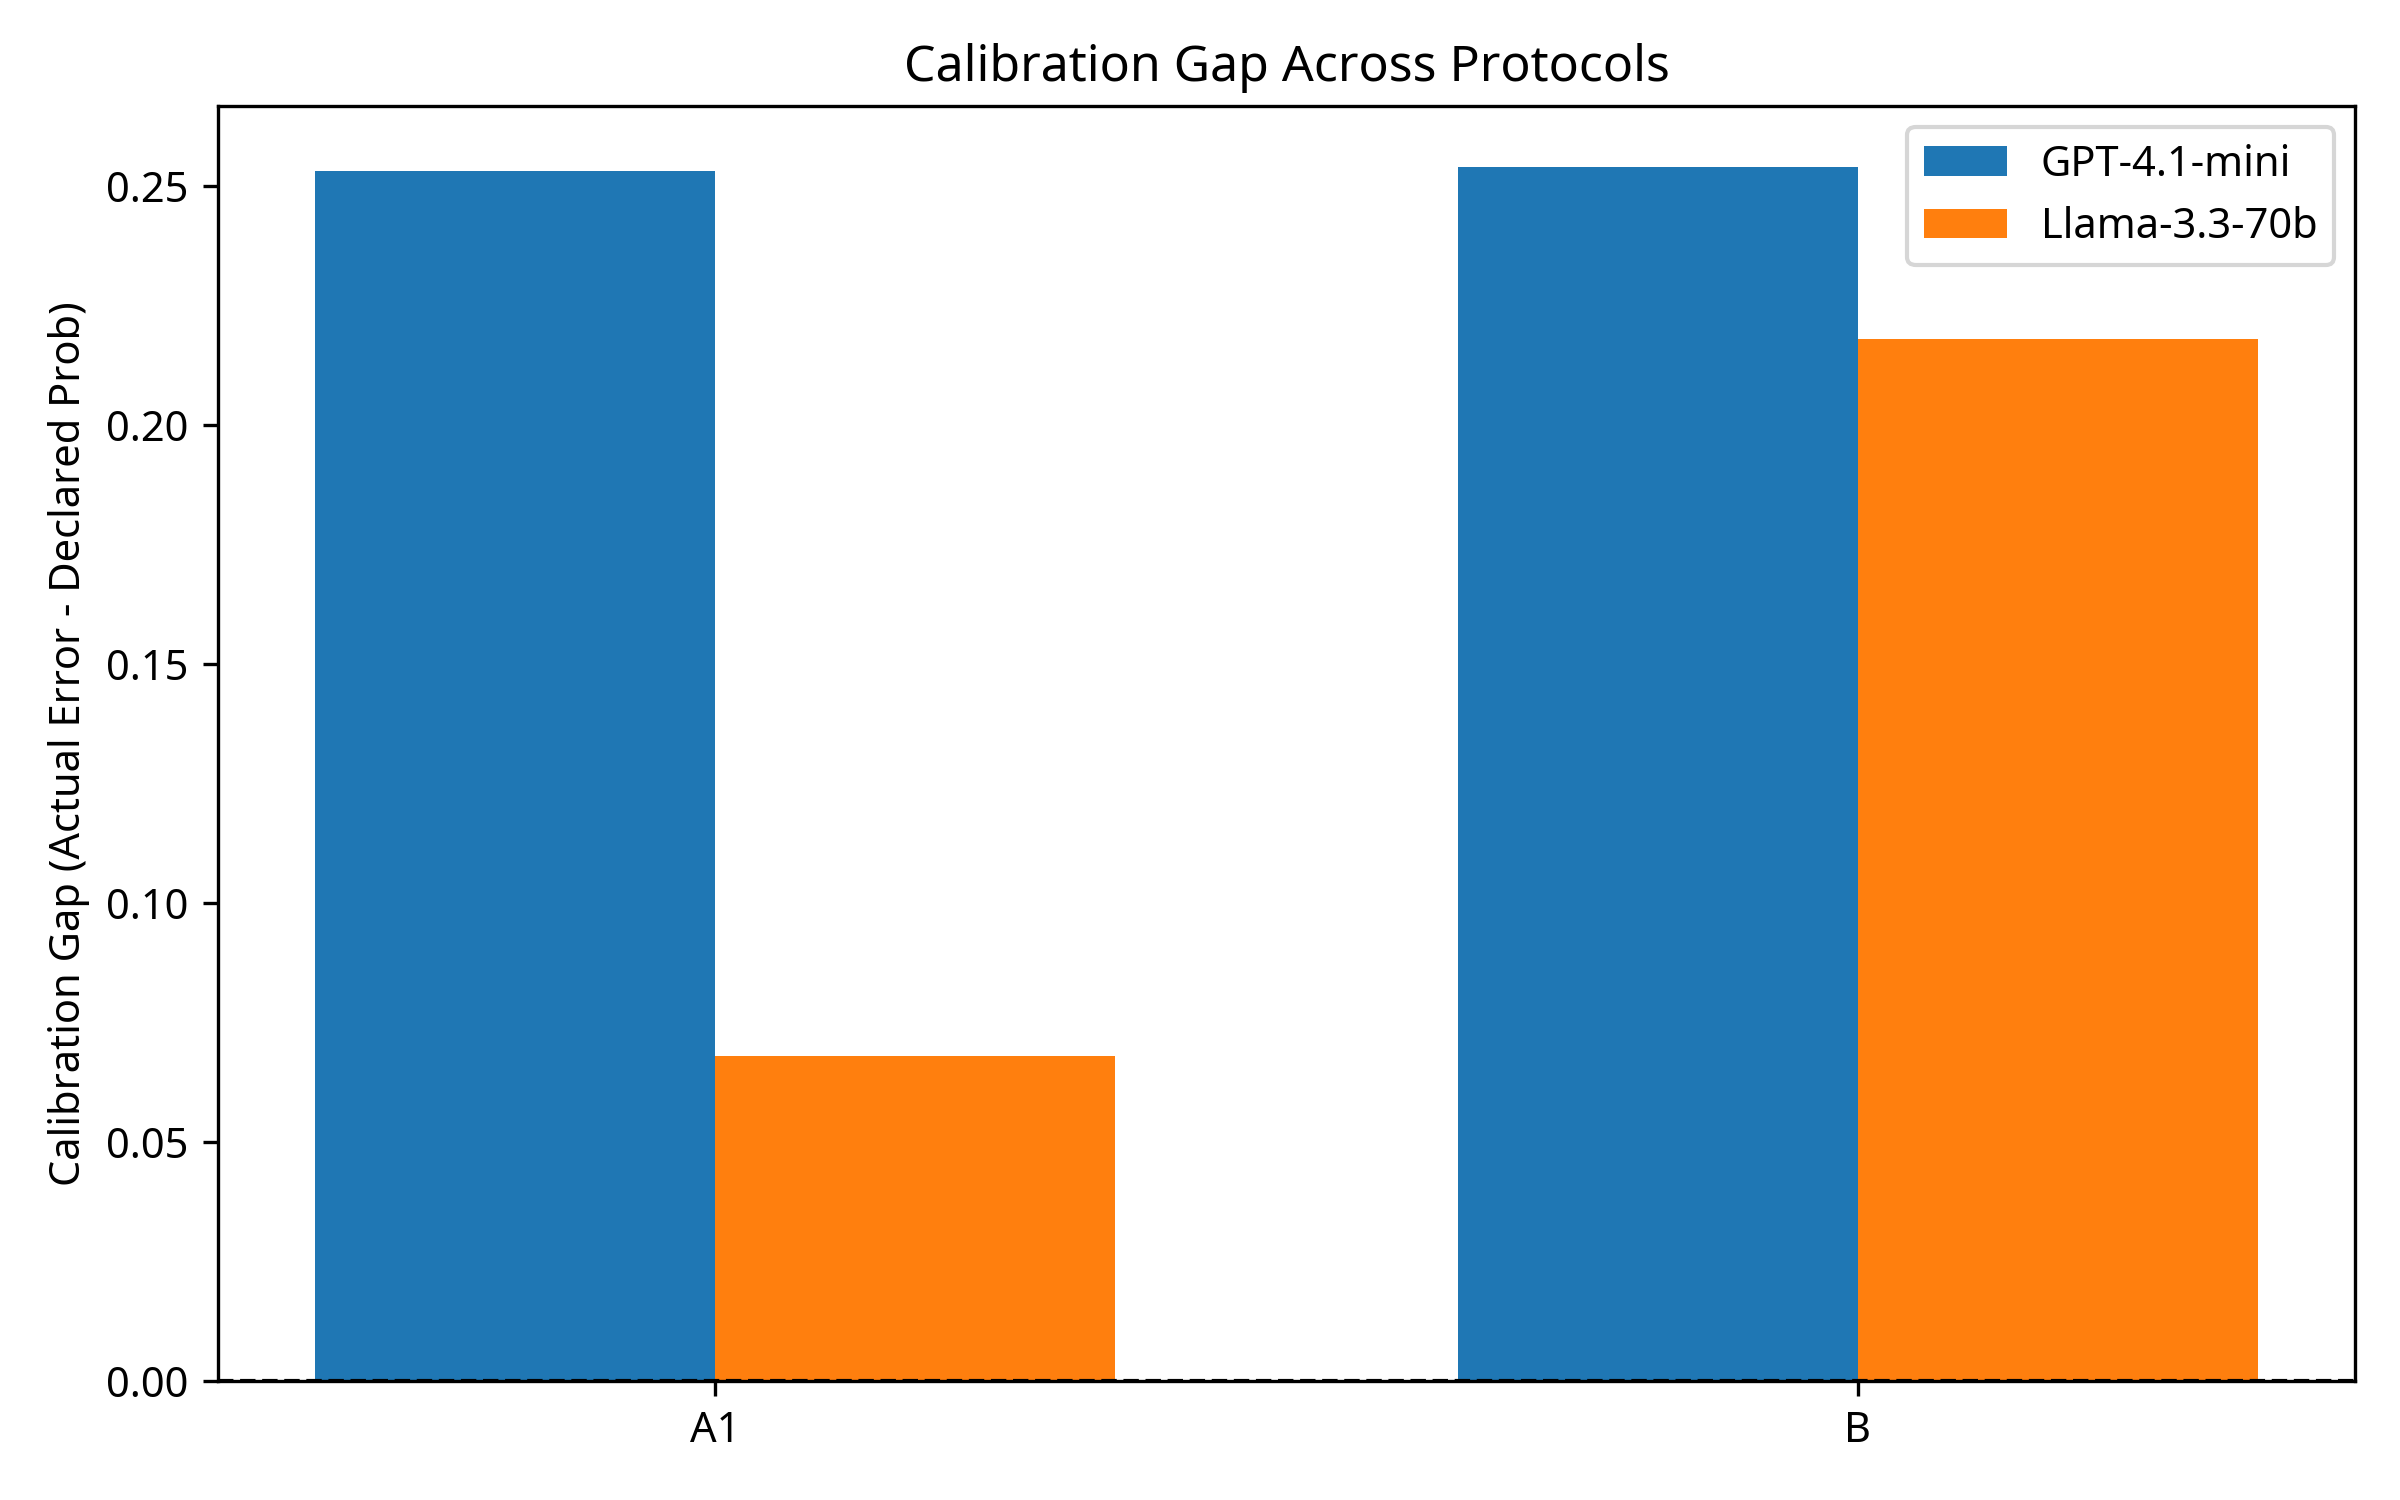
\includegraphics[width=\linewidth]{fig2_calibration_gap.png}
\caption{Calibration gap (actual error rate minus declared error probability) in Protocol B.}
\label{fig:calibration}
\end{figure}

\section{Reporting Checklist}
\begin{enumerate}
    \item \textbf{Data:} PubMedQA (MIT License).
    \item \textbf{Models:} GPT-4.1-mini, Llama-3.3-70b.
    \item \textbf{Compute:} API access, $\sim$\$15 total cost.
    \item \textbf{Hyperparameters:} Temperature 0.0, \texttt{max\_tokens} 80/300.
    \item \textbf{Metrics:} Accuracy, Cohen's $\kappa$, Calibration Gap.
    \item \textbf{Code:} Available at anonymous URL.
\end{enumerate}

\section{Discussion}

Our findings demonstrate that pipeline choices can manufacture the very metacognitive behaviors they intend to measure. The truncation artifact (Finding 1) highlights the danger of silent parser defaults. The tautological compliance (Finding 3) shows that explicit instructions can override intrinsic model behavior, creating an illusion of perfect calibration.

Crucially, the monitoring stage (error probability estimation) remains relatively stable, while the control stage (action selection) is highly malleable. The massive shift in abstention rates driven by evidence length (Finding 2) underscores that models are reacting to the context window rather than their own internal uncertainty.

\section{Limitations}
\begin{itemize}
    \item We evaluate only two models; results may differ for others.
    \item We use a single dataset (PubMedQA).
    \item We do not evaluate human baselines.
    \item We focus on zero-shot prompting without fine-tuning.
    \item The Arm D condition (prefix branching) was not run due to compute constraints.
\end{itemize}

\section{Conclusion}
Metacognitive evaluations must rigorously isolate pipeline artifacts. When models appear perfectly calibrated, researchers must ask whether the model is truly self-aware, or simply following the prompt.

\bibliography{custom}

\end{document}

